\chapter{Background}
This chapter describes state of the art concepts and algorithms, which were studied and used during this thesis. The background is divided into three sections.

Firstly grammars, which can be used to analyse or generate street networks are discussed. In that section \textit{Shape Grammars}, \textit{L-Systems} and the theory \textit{Space Syntax} are described and analysed.

Secondly the application CPlan is used to create and analyse cities. For this thesis it was extended with many algorithms.

Thirdly clustering algorithms are explained. Those unsupervised machine learning algorithms have the purpose to separate data with specific characteristics into meaningful groups. In this section the clustering algorithms K-Means and hierarchical clustering (Single-Linkage, WPGMA, UPGMA) are discussed. In later chapters the usage and implementation of those algorithms will be explained.

Lastly street networks measurement methods, that allow to analyse and compare street subgraphs are described.

\section{Shape Grammars} \label{sec:shape_grammar}
The main key of a shape grammars is to generate paintings by a new defined grammar based on shapes, selection rules, painting rules and limiting shapes. A shape grammar is a language based on an alphabet of shapes and generated shapes \citep{shapeGrammars:1972}.

A class of paintings defines the pair (S,M). S represents the shape specifications and M the material specifications. The shape specification contains a shape grammar, defining a language of two dimensional shapes, and a selection rule. M specifies a finite list of material specifications and one limiting shape on a canvas.

\subsection{Shape Grammar Definition}
\label{sec:Shape_Grammar_Definition}
A Shape Grammar is defined over an alphabet of shapes and generated n-dimensional shapes according to \citep{shapeGrammars:1972}.
\begin{quote} 
    Definition. A shape grammar (SG) is a 4-tuple: $SG = (V_T, V_M, R, I)$ where
    \begin{enumerate}
        \item $V_T$ is a finite set of shapes.
        \item $V_M$ is a finite set of shapes such that $V_T $* $\cap$  $V_M = \emptyset$
        \item R is a finite set of ordered pairs (u,v) such that
        
        u is a shape consisting of an element of $V_T $* combined with an element of $V_M$ and
        
        v is a shape consisting of (A) the element of $V_T $* contained in u or (B) the element of $V_T $* contained in u combined with an element of $V_M$ or (C) the element of $V_T $* contained in u with an additional element of $V_T$* and an element of $V_M$.
        
        \item I is a shape consisting of elements of $V_T $* and $V_M$.
    \end{enumerate}
\end{quote}

\subsection{Selection Rules}
\label{sec:Shape_Grammar_Selection_Rules}
A painting is generated based on an undefined count of shape rules. This requires a mechanism to select a correct shape. The depth is defined by levels which are being assigned during generation based on their rules according to \citep{shapeGrammars:1972}:
\begin{displayquote}
    \begin{enumerate}
        \item The terminals in the initial shape are assigned to level 0.
        \item If a shape rule is applied, and the highest level assigned to any part ot the terminal corresponding to the level side of the rule is N, then
        \begin{enumerate}
            \item If the rule is of type A, any part of the terminal enclosed by the marker in the left side of the rule is assigned to N.
            \item If the rule is of type B, any part of the terminal enclosed by the marker in the left side of the rule is assigned to N and any part of the terminal enclosed by the marker is assigned to N+1.
            \item If the rule is of type C, the terminal added is assigned to N+1.
        \end{enumerate}
        \item No other level assignments are made.
    \end{enumerate}
\end{displayquote}

\subsection{Painting Rules}
\label{sec:Shape_Grammar_Painting_Rules}
Painting rules describe witch shape should be painted inside of a defined area. Like in a Venn diagram the rules contain multiple levels 0 - n. By combining these levels the painting colour is described\citep{shapeGrammars:1972}. The assignments are made by the common operators. An example can be viewed in figure \ref{fig:shape_grammar_gen_specifications}

\subsection{Limiting Shapes}
\label{sec:Shape_Grammar_Limiting_Shapes}
These shapes define a limiting area on the canvas, where shape painting is allowed. 
The area could have any form, but normally it is defined as a rectangle. Like a camera view the limiting shape defines the scale of a painting and its viewpoint. Therefore the initial/start shape could be outside of the limiting shape.

\subsection{Example}
These specifications \ref{fig:shape_grammar_gen_specifications} have been used to generate the output image \ref{fig:Shape Grammars/Example}.

In the output image \ref{fig:Shape Grammars/Example} the relevant steps can be observed. The levels are generated as described in the section \ref{sec:Shape_Grammar_Selection_Rules}.
\newline
Level 0 is represented by steps 0 and 1. Steps 2 to 5 are on level 1 and finally steps 18 and 19 are on Level 2.
\begin{figure}[!ht]
    \centering
    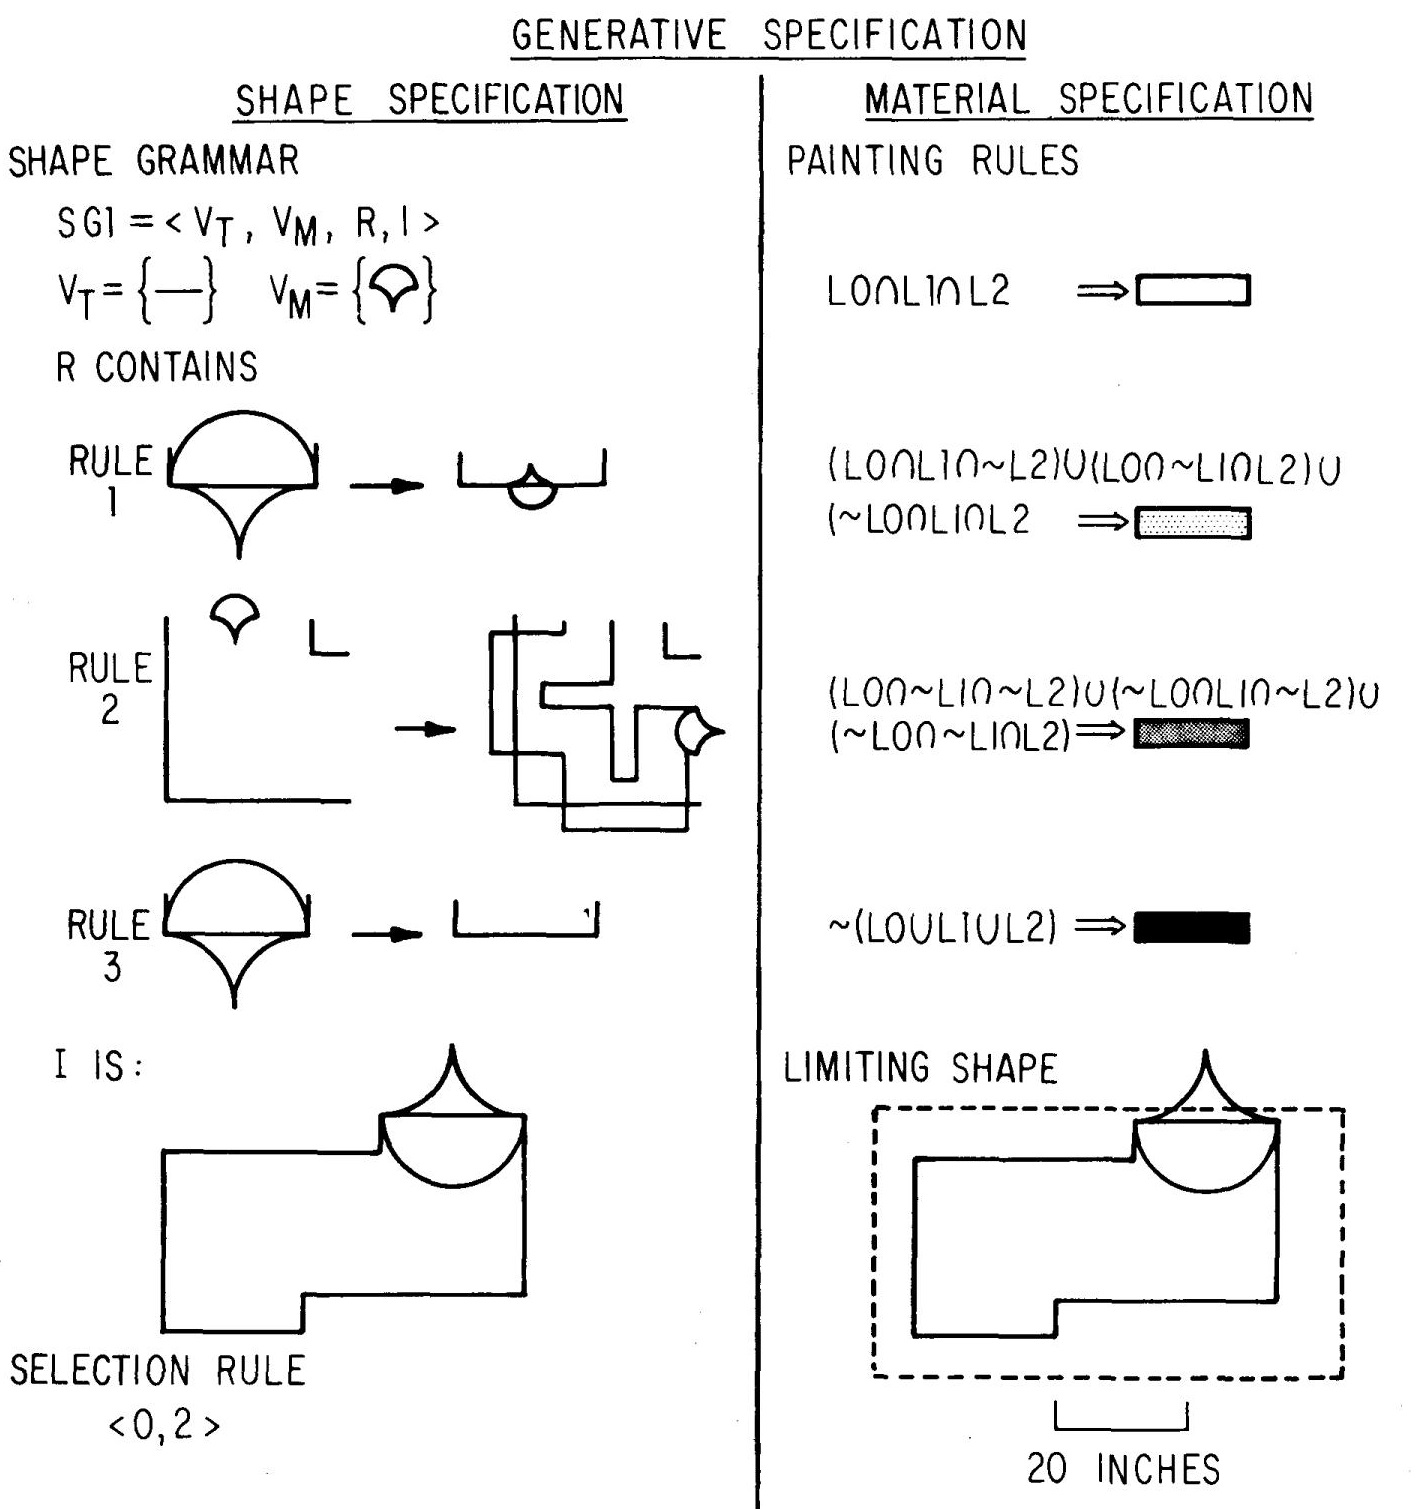
\includegraphics{shape_grammar_generativ_spec.jpg}
    \caption{Generative Specifications - \textit{Source: Shape Grammar} \citep{shapeGrammars:1972}}
    \label{fig:shape_grammar_gen_specifications}
\end{figure}

\begin{figure}[!ht]
    \centering
    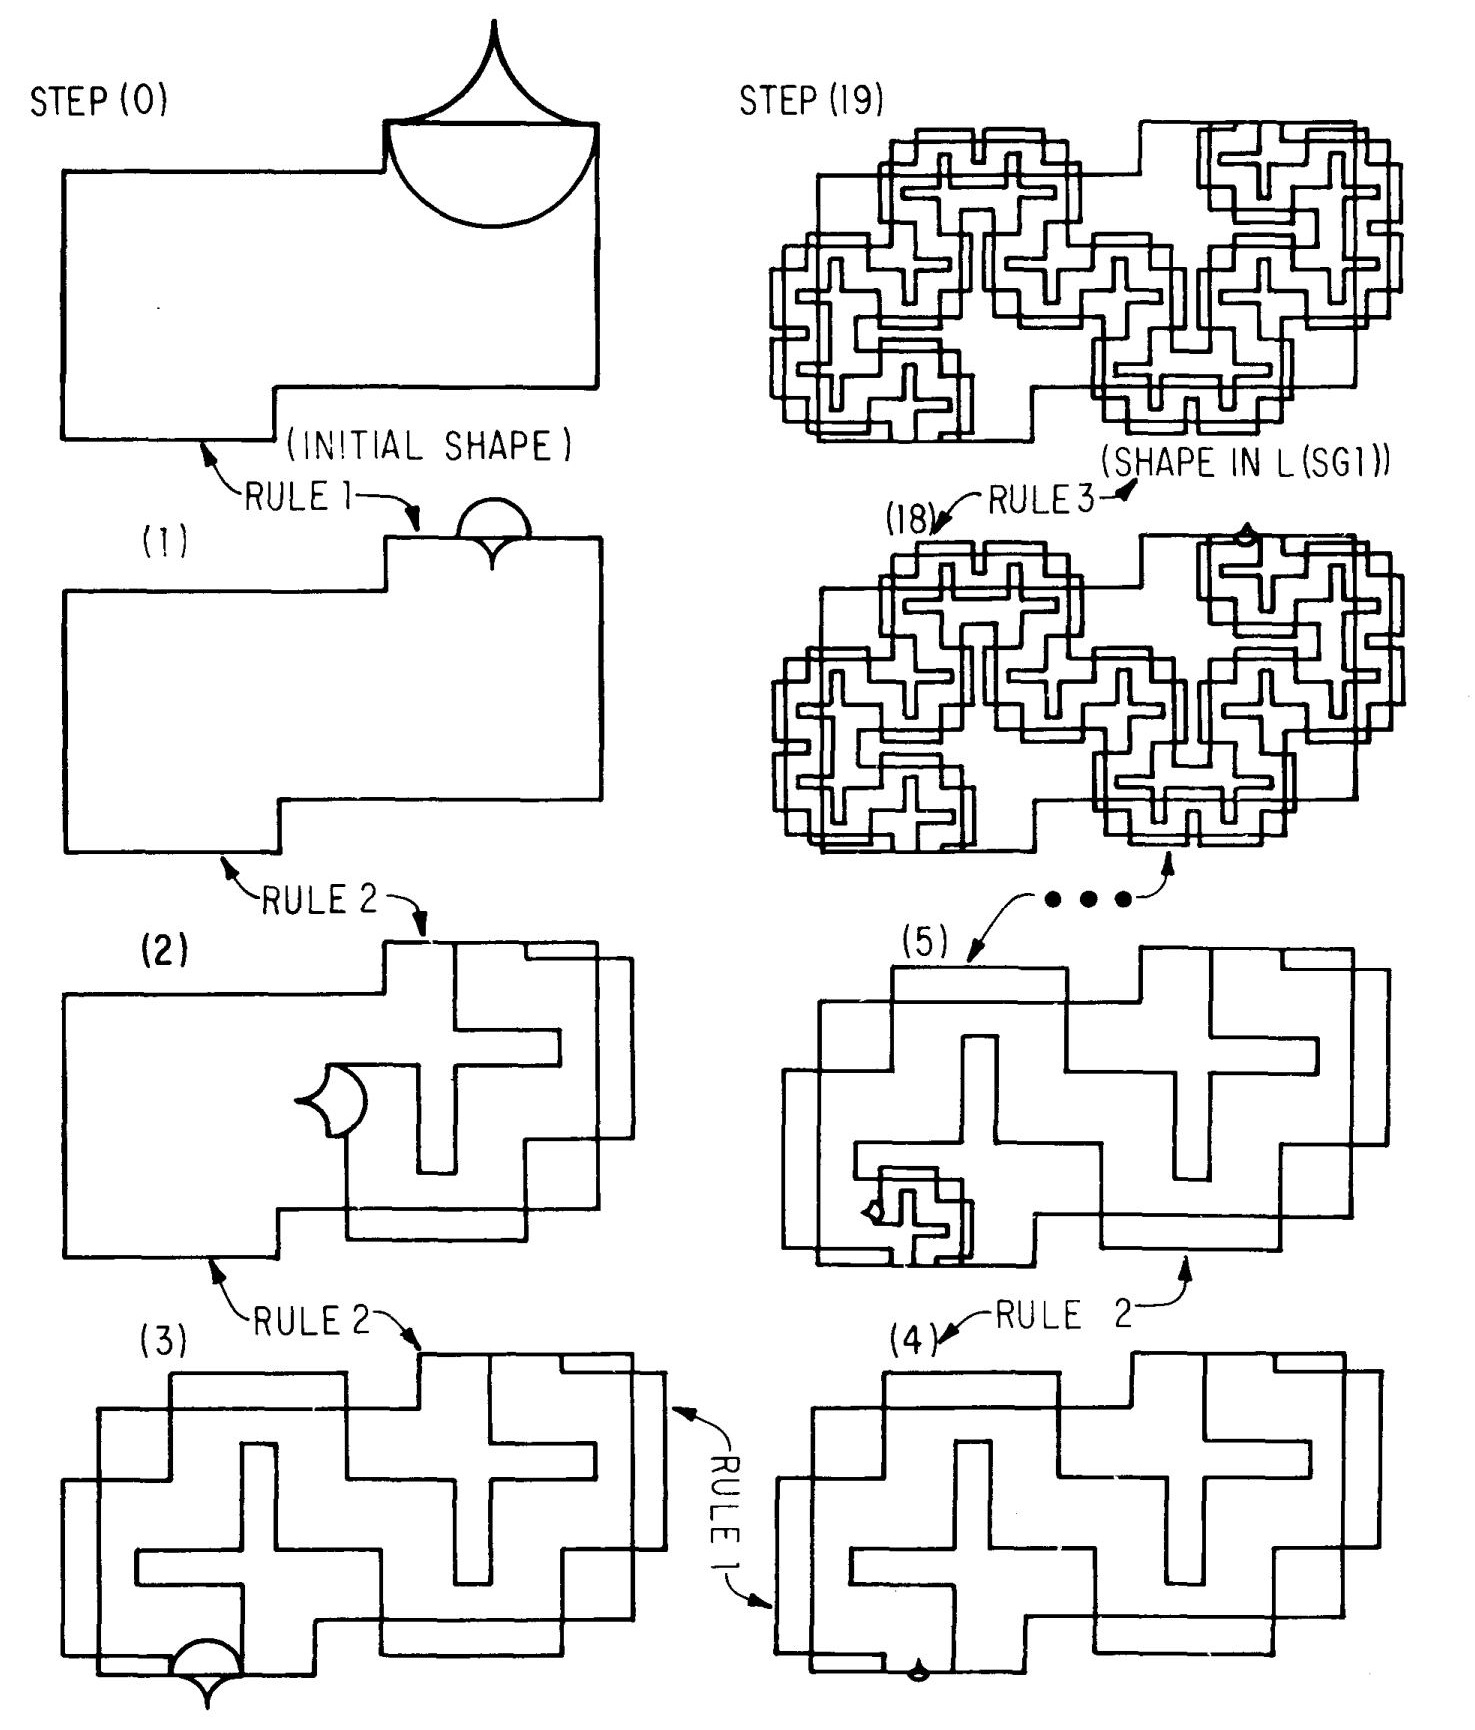
\includegraphics[width=\textwidth]{sg_example.jpg}
    \caption{ Generated Painting - \textit{Source: Shape Grammar} \citep{shapeGrammars:1972}}
    \label{fig:Shape Grammars/Example}
\end{figure}

\FloatBarrier
\pagebreak
\subsection{Street Generation}
In the following section we debate the usefulness of generating street networks by shape grammars.
\subsubsection{Features}
\begin{itemize}
    \item Can describe and generate veneer in high details.
    \item With R-Shapes windows and high detail 3D-Models can be generated easily.
\end{itemize}

\subsubsection{Problems}
\begin{itemize}
    \item The given methods generate monotonous streets in most cases. 
    \item A huge number of R-Shapes is required to generate a useful street network.
    \item Areas with different characteristics (historic district, rectangular raster like New York or radial to center like Paris) are difficult to generate.
    \item The R-Rules for the transitions between area characteristics should not repeat themselves and are for that reason difficult to build.
\end{itemize}

\pagebreak
\section{L-Systems} \label{sec:L-Systems}
L-System is a well established modelling approach for the synthesis of realistic plant images. There are many papers describing L-Systems and how they are applied to generate plant life: "In these cases L-System productions capture the \textit{development} of plant components over time." \citep{PrusinkiewiczEtAl:2001} Productions are applied in parallel, so that all plant parts grow and age equally. The growth is stopped at a defined terminal age. This age is the number of iterations, where in each iteration productions are applied.

The context-free productions in \citep{PrusinkiewiczEtAl:2001} are defined using the following syntax.
\begin{equation} \label{eq:lsystem context free}
pred : \{block1\}\ cond\ \{block2\} \leadsto succ
\end{equation}
The symbol \textit{pred} (predecessor) defines the module that will get replaced by the modules defined in \textit{succ} (successor). This replacement is only applied, if the (optional) condition is met. \textit{block1} and \textit{block2} are C statement blocks, of which the first block is executed before and the second after the condition is evaluated. \citep{PrusinkiewiczEtAl:2001} gives the following example.
\begin{equation} \label{eq:lsystem example 1}
A(x) : \{y = x + 2;\}\ y \geq 5\ \{z = y / 3;\}\ \leadsto B(z)C(z + 1)
\end{equation}
If this example production was applied to the module $A(4)$, it would result in the modules $B(2)C(3)$.

The modelling language, described in \citep{PrusinkiewiczEtAl:2001}, also supports context-sensitive productions. The following listing defines the syntax of such a production.
\begin{equation} \label{eq:lsystem context sensitive}
lcont < pred > rcont : \{block1\}\ cond\ \{block2\} \leadsto succ
\end{equation}
\textit{lcont} (left context) and \textit{rcont} (right context) each define a list of modules that have to precede or respectively follow the \textit{pred} (module being replaced). Context modules are limited to query symbols, which are explained later on. \citep{PrusinkiewiczEtAl:2001} gives the following example.
\begin{equation} \label{eq:lsystem example 2}
A(x) < B(y) > C(z) : x + z > 0 \leadsto M(y / 2)N(y / 2)
\end{equation}
If the example of listing \ref{eq:lsystem example 2} was applied to the module composition $A(2)B(4)C(0)$, it would result in the modules $A(2)M(2)N(2)C(0)$.

A way to generate images with L-Systems is to use a LOGO-style turtle as a graphical model. Certain modules of the L-System are interpreted as commands to this turtle.

\pagebreak
\section{Space Syntax} \label{sec:space_syntax}
The axial line-based space syntax was first introduced in 1976 by B. Hiller, A. Leaman, P. Stansall and M. Bedford in the paper \textit{Space syntax} \citep{spaceSyntax:1976}. This theory is based on a morphic language and describes methods to analyse and generate urban areas and buildings.

The theory was later extended and integrated into \textit{Geographic Information System} (GIS) as point-based space syntax (graph). This systems are used to plan and analyse the human interaction with the environment.

\subsection{Axial line-based space syntax and limitations}
In space syntax streets are represented by axial lines. 
\textit{"Axial lines are used to represent directions of uninterrupted movement and visibility, so they represent the longest visibility lines in two-dimensional urban spaces."} \citep{integrationSpaceSyntaxGIS:2002}
This approach has allowed many analysis methods of urban systems like way-finding process or criminal analysis. An axial map represents a fully filled free space with many axial lines \ref{fig:barnsbury_axial_map}. For a more detailed analysis the lines can by broken into segments at the intersections \ref{fig:barnsbury_segmented_axial_map}. To generate the axial map always the longest not visited space is selected and line drawn till the hole space is covered.

Axial maps have many limitations. First the complexity to create an axial map is high because of the generating procedure. If an additional area is added the hole process of detection should be repeated because a longer start line could exist. The process is non-deterministic because a curve could be separated into a unknown count of lines.

\begin{figure}[ht]
    \centering
    \begin{subfigure}[b]{0.4\textwidth}
        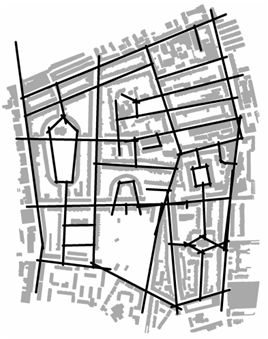
\includegraphics[width=\textwidth]{The-figure-ground-plan-of-Barnsbury-Axial-map.jpg}
        \caption{Barnsbury axial map}
        \label{fig:barnsbury_axial_map}
    \end{subfigure}
    \quad
    \begin{subfigure}[b]{0.4\textwidth}
        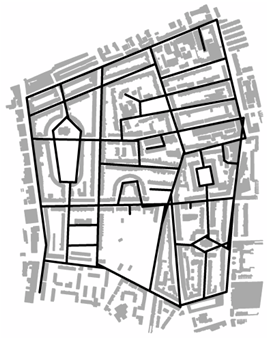
\includegraphics[width=\textwidth]{The-figure-ground-plan-of-Barnsbury-Axial-segment-map.jpg}
        \caption{Barnsbury segmented axial map}
        \label{fig:barnsbury_segmented_axial_map}
    \end{subfigure}
    \caption{Space Syntax: Axial Map - \textit{Source: UCL Space Syntax \citep{SpaceSyntaxExampels}}}
    \label{fig:SpaceSyntaxAxialMap}
\end{figure}

\subsection{Point-based space syntax}
A point-based space syntax is a decision based approach as described by Bin Jiang and Christope Claramunt in \textit{Integration of Space Syntax into GIS: New Perspectives for Urban Morphology} \citep{integrationSpaceSyntaxGIS:2002}. Every time a point in a street network is visited the visitor can decide which direction he will travel next. The distances between two point can directly be measured and described. Every point can be assigned to an ID and marked with x and y coordinates \ref{fig:space_syntax_gis_characteristic_points}. This approach is at least equivalent to the predefined syntax created by B. Hiller et al.\citep{spaceSyntax:1976} because a visibility graph can be create to represent axial lines \ref{fig:space_syntax_gis_visibility_graph}. The point-based space syntax therefore is a graph based approach.

\begin{figure}[ht]
    \centering
    \begin{subfigure}[b]{0.4\textwidth}
        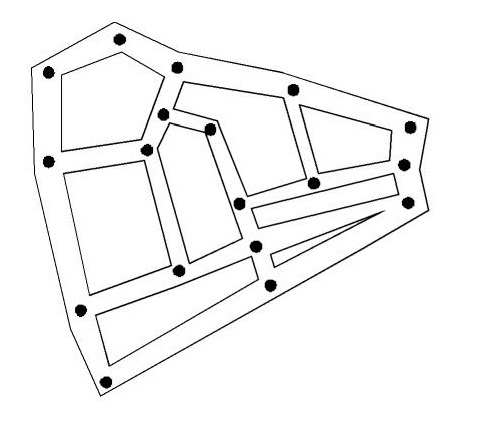
\includegraphics[width=\textwidth]{space_syntax_gis_characteristic_points.jpg}
        \caption{Characteristic points}
        \label{fig:space_syntax_gis_characteristic_points}
    \end{subfigure}
    \quad
    \begin{subfigure}[b]{0.4\textwidth}
        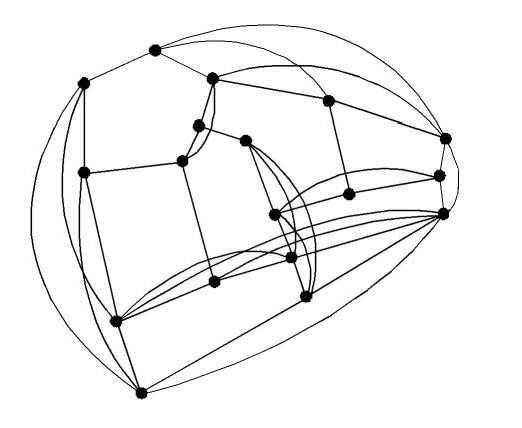
\includegraphics[width=\textwidth]{space_syntax_gis_visibility_graph.jpg}
        \caption{Visibility graph}
        \label{fig:space_syntax_gis_visibility_graph}
    \end{subfigure}
    \caption{Point-based space syntax - \textit{Source: Integration of Space Syntax into GIS \citep{integrationSpaceSyntaxGIS:2002}}}
    \label{fig:space_syntax_gis}
\end{figure}

\subsection{Comparison with CPlan}
The application CPlan \ref{CPlan} does handle the street networks as graphs. As a result the same measurements methods can be applied as described for the point-based space syntax. The clustering algorithms later discussed \ref{sec:K-Means}, \ref{sec:hierarchicalClustering} are based on vertex/points and unidirectional edges between the points.